\documentclass[11pt]{article}
\usepackage{amsmath} % For math symbols
\usepackage{amssymb} % For checkmark and other symbols
\usepackage{array} % For better tables
\usepackage{booktabs} % For professional-looking tables
\usepackage{graphicx}
\usepackage{float}      % for [H] placement
\usepackage{xcolor,colortbl}  % for row colors


\title{COMS 4733 Homework 2}
\author{Jaisel Singh}
\date{\today}
\begin{document}
\maketitle
\section{Problem 1: Discrete Search Algorithms}
\subsection{Search Algorithm Comparison}
% Define notation
\noindent\textbf{Notation:}
\begin{itemize}
\item $b$ = branching factor (average number of successors per node)
\item $d$ = depth of the shallowest goal node
\item $m$ = maximum depth of the search tree
\end{itemize}
\noindent\textit{Note: All algorithms use graph search (visited set) on finite state space.}

\begin{table}[h]
\centering
\begin{tabular}{|l|c|c|c|c|}
\hline
\textbf{Algorithm} & \textbf{Complete?} & \textbf{Cost-Optimal?} & \textbf{Time Complexity} & \textbf{Space Complexity} \\
\hline
DFS & Yes & No & $O(b^m)$ or $O(V + E)$ & $O(bm)$ or $O(V)$ \\
\hline
BFS & Yes & No & $O(b^d)$ or $O(V + E)$ & $O(b^d)$ or $O(V)$ \\
\hline
Dijkstra & Yes & Yes & $O(b^d)$ or $O((V + E)\log(V))$ & $O(b^d)$ or $O(V)$ \\
\hline
A* (admissible $h$) & Yes & Yes & $O(b^d)$ & $O(b^d)$ \\
\hline
\end{tabular}
\caption{Comparison of search algorithms}
\label{tab:search_comparison}
\end{table}

\subsubsection*{Justification for Selected Entries}

\textbf{Dijkstra's Algorithm - Time Complexity: $O(b^d)$}

Dijkstra's algorithm explores nodes in order of increasing cost from the start node. In the worst case, it must explore all nodes up to the depth $d$ of the optimal solution before guaranteeing it has found the cheapest path.

Consider a tree structure where:
\begin{itemize}
\item At depth 0: 1 node (start)
\item At depth 1: $b$ nodes
\item At depth 2: $b^2$ nodes
\item $\vdots$
\item At depth $d$: $b^d$ nodes
\end{itemize}

The total number of nodes explored is:
$$1 + b + b^2 + \cdots + b^d = \frac{b^{d+1} - 1}{b - 1} = O(b^d)$$

Each node is processed once (removed from the priority queue), and for each of its neighbors, we may perform a priority queue operation. With an efficient priority queue implementation (binary heap), these operations take $O(\log n)$ time where $n$ is the number of nodes in the queue.

Therefore, the overall time complexity is $O(b^d)$ in the context of search algorithms.

\textbf{Dijkstra's Algorithm - Space Complexity: $O(b^d)$}

Dijkstra's algorithm uses a priority queue to store nodes that have been discovered but not yet fully explored. In the worst case, before reaching the goal at depth $d$, the priority queue may contain all nodes at the frontier of the search.

Since Dijkstra's explores in a breadth-first manner (ordered by cost rather than depth), it must maintain all nodes at the current cost level. In a tree with branching factor $b$ and goal at depth $d$, the maximum number of nodes in the priority queue at once is proportional to $b^d$ (the number of nodes at depth $d$).

Additionally, with graph search (using a visited set to avoid cycles), we must store all visited nodes, which is also $O(b^d)$ in the worst case.

Therefore, the space complexity is $O(b^d)$.

\subsection{Search Tree Expansion}

\subsubsection{Task 1: BFS Expansion Order}

Using lexicographic ordering (smallest $x$ first, then smallest $y$) for tie-breaking, the BFS expansion order is:

\begin{center}
\begin{tabular}{|c|c|c|c|}
\hline
\textbf{(0,3)} & \textbf{(1,3)} & \textbf{(2,3)} & \textbf{G (3,3)} \\
5 & 8 & 12 & 14 \\
\hline
\textbf{(0,2)} & \textbf{X (1,2)} & \textbf{(2,2)} & \textbf{(3,2)} \\
2 & - & 9 & 13 \\
\hline
\textbf{S (0,1)} & \textbf{(1,1)} & \textbf{(2,1)} & \textbf{(3,1)} \\
0 & 3 & 6 & 10 \\
\hline
\textbf{(0,0)} & \textbf{(1,0)} & \textbf{(2,0)} & \textbf{(3,0)} \\
1 & 4 & 7 & 11 \\
\hline
\end{tabular}
\end{center}

\textbf{Complete expansion sequence:}
\begin{align*}
&0: S(0,1) \rightarrow 1: (0,0) \rightarrow 2: (0,2) \rightarrow 3: (1,1) \rightarrow 4: (1,0) \rightarrow 5: (0,3) \rightarrow 6: (2,1) \\
&\rightarrow 7: (2,0) \rightarrow 8: (1,3) \rightarrow 9: (2,2) \rightarrow 10: (3,1) \rightarrow 11: (3,0) \rightarrow 12: (2,3) \\
&\rightarrow 13: (3,2) \rightarrow 14: G(3,3)
\end{align*}

\subsubsection{Task 2: Dijkstra's Algorithm}

Dijkstra's algorithm expands nodes in the \textbf{same order} as BFS for this problem.

\textbf{Explanation:} 

BFS and Dijkstra's expand nodes identically because all edges have uniform cost (cost = 1). Dijkstra's algorithm uses a priority queue to explore nodes in order of increasing cumulative cost from the start. Since each move costs 1, a node at distance $d$ from the start has total cost $d$. This matches BFS exactly, which explores nodes layer-by-layer by distance.

When multiple nodes have the same priority (same cost in Dijkstra's, same depth in BFS), both algorithms apply the lexicographic tie-breaking rule. Since cost equals depth in this uniform-cost scenario, both algorithms break ties identically and produce the same expansion order.

Therefore, Dijkstra's expansion order is identical to the BFS grid shown above.

\subsubsection{Task 3: A* with Manhattan Distance Heuristic}

Using the Manhattan distance heuristic $h(x,y) = |3-x| + |3-y|$ and lexicographic tie-breaking, A* expands nodes in the following order:

\begin{center}
\begin{tabular}{|c|c|c|c|c|}
\hline
\textbf{Order} & \textbf{Node} & \textbf{$g(n)$} & \textbf{$h(n)$} & \textbf{$f(n) = g(n) + h(n)$} \\
\hline
0 & S (0,1) & 0 & 5 & 5 \\
\hline
1 & (0,2) & 1 & 4 & 5 \\
\hline
2 & (0,3) & 2 & 3 & 5 \\
\hline
3 & (1,1) & 1 & 4 & 5 \\
\hline
4 & (1,3) & 3 & 2 & 5 \\
\hline
5 & (2,1) & 2 & 3 & 5 \\
\hline
6 & (2,2) & 3 & 2 & 5 \\
\hline
7 & (2,3) & 4 & 1 & 5 \\
\hline
8 & (3,1) & 3 & 2 & 5 \\
\hline
9 & (3,2) & 4 & 1 & 5 \\
\hline
10 & G (3,3) & 5 & 0 & 5 \\
\hline
\end{tabular}
\end{center}

\textbf{Grid with expansion order:}

\begin{center}
\begin{tabular}{|c|c|c|c|}
\hline
\textbf{(0,3)} & \textbf{(1,3)} & \textbf{(2,3)} & \textbf{G (3,3)} \\
2 & 4 & 7 & 10 \\
\hline
\textbf{(0,2)} & \textbf{X (1,2)} & \textbf{(2,2)} & \textbf{(3,2)} \\
1 & - & 6 & 9 \\
\hline
\textbf{S (0,1)} & \textbf{(1,1)} & \textbf{(2,1)} & \textbf{(3,1)} \\
0 & 3 & 5 & 8 \\
\hline
\textbf{(0,0)} & \textbf{(1,0)} & \textbf{(2,0)} & \textbf{(3,0)} \\
- & - & - & - \\
\hline
\end{tabular}
\end{center}

\textbf{Observations/Notes}

\begin{itemize}
    \item All expanded nodes have $f(n) = 5$, which equals the optimal path cost
    \item Nodes in row $y=0$ (bottom row) such as (0,0), (1,0), (2,0), and (3,0) are generated but never expanded because they all have $f = 7 > 5$
    \item The Manhattan distance heuristic is admissible (never overestimates) and consistent in this 4-connected grid with unit costs
    \item Because $h$ is admissible and the grid uses 4-connected movement with unit costs, every node on an optimal path satisfies $g + h = 5$ (constant). Therefore, the expansion order among these nodes is determined purely by the lexicographic tie-breaking rule
    \item A* reaches the goal at step 10, having expanded only 11 nodes (including the start), compared to 15 nodes for BFS
\end{itemize}

\subsection{Heuristic Admissibility}

\subsubsection*{Is Euclidean distance admissible?}

\textbf{Answer:} Yes, the Euclidean distance heuristic $h(n) = \sqrt{(x_g - x)^2 + (y_g - y)^2}$ is admissible for this cost model.

\textbf{Justification:}

A heuristic is admissible if it never overestimates the true optimal cost to reach the goal. The Euclidean distance represents the straight-line distance between two points, which is the shortest possible distance in Euclidean space.

With 8-connected movement where diagonal moves cost $\sqrt{2}$ and cardinal moves cost 1, we can analyze the relationship between the heuristic and actual cost:

\begin{itemize}
    \item Consider moving from $(0,0)$ to $(3,3)$:
    \begin{itemize}
        \item Euclidean distance: $h = \sqrt{(3-0)^2 + (3-0)^2} = \sqrt{18} = 3\sqrt{2} \approx 4.243$
        \item Optimal path: Three diagonal moves $(0,0) \rightarrow (1,1) \rightarrow (2,2) \rightarrow (3,3)$
        \item Actual cost: $3\sqrt{2} \approx 4.243$
    \end{itemize}
    \item In general, for any two points, the Euclidean distance equals the cost of moving in a straight diagonal line (when possible), which is the optimal path in an obstacle-free 8-connected grid
    \item Since we cannot move "more directly" than the straight line, and diagonal moves have cost exactly $\sqrt{2}$, the Euclidean distance never overestimates the true cost
\end{itemize}

Therefore, the Euclidean distance heuristic is admissible for this cost model.

\subsubsection*{Propose a different admissible heuristic}

\textbf{Answer:} The Chebyshev distance (L$^\infty$ norm) is an admissible heuristic for this cost model:
$$h(n) = \max(|x_g - x|, |y_g - y|)$$

\textbf{Justification:}

The Chebyshev distance measures the maximum absolute difference in either coordinate, which corresponds to the minimum number of moves required to reach the goal when diagonal moves are allowed.

To show admissibility, we verify that this heuristic never overestimates:

\begin{itemize}
    \item The Chebyshev distance counts the number of diagonal or cardinal moves needed along the longer dimension
    \item Example: From $(0,0)$ to $(3,3)$:
    \begin{itemize}
        \item Chebyshev distance: $h = \max(|3-0|, |3-0|) = 3$
        \item Optimal path: Three diagonal moves with cost $3\sqrt{2} \approx 4.24$
        \item Since $3 < 4.24$, the heuristic does not overestimate
    \end{itemize}
    \item More generally, consider moving from $(x, y)$ to $(x_g, y_g)$:
    \begin{itemize}
        \item Let $\Delta x = |x_g - x|$ and $\Delta y = |y_g - y|$
        \item Assume without loss of generality that $\Delta x \geq \Delta y$
        \item Optimal strategy: Move diagonally $\Delta y$ times, then cardinally $(\Delta x - \Delta y)$ times
        \item Actual cost: $\Delta y \cdot \sqrt{2} + (\Delta x - \Delta y) \cdot 1 = \Delta x + \Delta y(\sqrt{2} - 1)$
        \item Chebyshev distance: $h = \Delta x$
        \item Since $\sqrt{2} - 1 \approx 0.414 > 0$, we have $h = \Delta x < \Delta x + \Delta y(\sqrt{2} - 1)$ = actual cost
    \end{itemize}
\end{itemize}

Therefore, the Chebyshev distance never overestimates the true cost and is admissible.

\textbf{Alternative:} Any scaled Manhattan distance of the form $h(n) = c \cdot (|x_g - x| + |y_g - y|)$ where $c \leq \frac{\sqrt{2}}{2} \approx 0.707$ is also admissible, though it provides a looser bound than Chebyshev distance.

\subsection{PRM Construction and Search}

\subsubsection*{Task 1: Discard samples inside obstacle}

The obstacle is defined by corners at $(4,4)$ and $(6,6)$, forming a rectangle where $4 \leq x \leq 6$ and $4 \leq y \leq 6$.

Checking each sample:
\begin{itemize}
    \item $(2,2)$: Outside obstacle
    \item $(3,7)$: Outside obstacle
    \item $(5,2)$: Outside obstacle
    \item $(7,3)$: Outside obstacle
    \item $(8,5)$: Outside obstacle
    \item $(5,8)$: Outside obstacle
    \item $(3,3)$: Outside obstacle
    \item $(8,8)$: Outside obstacle
    \item $(5,5)$: \textbf{Inside obstacle - discarded}
\end{itemize}

\textbf{Result:} 8 valid samples remain after discarding $(5,5)$.

\subsubsection*{Task 2: Connect samples within radius $r = 2.5$}

Computing Euclidean distances between all pairs of valid samples (including start and goal), we connect pairs with distance $\leq 2.5$:

\textbf{Edges created:}
\begin{itemize}
    \item Start $(1,1)$ to $(2,2)$: $d = \sqrt{2} \approx 1.41$
    \item $(2,2)$ to $(3,3)$: $d = \sqrt{2} \approx 1.41$
    \item $(3,3)$ to $(5,2)$: $d = \sqrt{5} \approx 2.24$
    \item $(3,7)$ to $(5,8)$: $d = \sqrt{5} \approx 2.24$
    \item $(5,2)$ to $(7,3)$: $d = \sqrt{5} \approx 2.24$
    \item $(7,3)$ to $(8,5)$: $d = \sqrt{5} \approx 2.24$
    \item $(8,8)$ to Goal $(9,9)$: $d = \sqrt{2} \approx 1.41$
\end{itemize}

\subsubsection*{Task 3: Resulting roadmap}

The constructed PRM graph has two disconnected components:
\begin{itemize}
    \item \textbf{Left component:} Start $(1,1) \rightarrow (2,2) \rightarrow (3,3) \rightarrow (5,2) \rightarrow (7,3) \rightarrow (8,5)$ and $(3,7) \rightarrow (5,8)$
    \item \textbf{Right component:} $(8,8) \rightarrow$ Goal $(9,9)$
\end{itemize}

\begin{figure}[h]
    \centering
    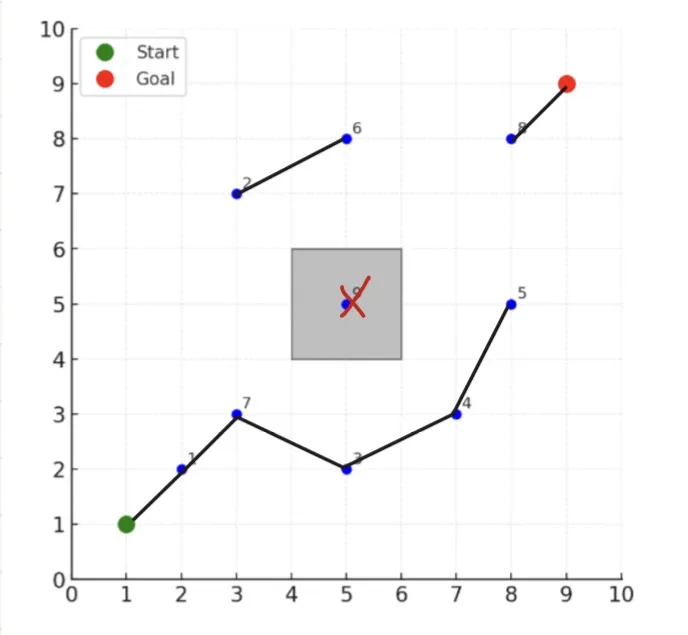
\includegraphics[width=0.6\textwidth]{roadmapimg.png}
    \caption{Constructed PRM roadmap showing valid samples (blue), start (green), goal (red), obstacle (gray), and edges connecting nodes within radius $r = 2.5$.}
    \label{fig:prm_roadmap}
\end{figure}


\subsubsection*{Task 4: Search algorithm}

Running Dijkstra's algorithm from Start $(1,1)$:

The algorithm explores all nodes reachable from the start but cannot reach the goal because the graph is disconnected. The search terminates without finding a path.

\subsubsection*{Task 5: Results and connectivity analysis}

\textbf{Path length:} No path exists.

\textbf{Number of nodes expanded:} Dijkstra's expands all nodes in the connected component containing the start: Start, $(2,2)$, $(3,3)$, $(3,7)$, $(5,2)$, $(5,8)$, $(7,3)$, $(8,5)$ = 8 nodes.

\textbf{Explanation:} The PRM fails to find a path because the roadmap is disconnected. The obstacle at $(4,4)$ to $(6,6)$ combined with the connection radius $r = 2.5$ creates a gap that prevents connectivity between the left and right sides of the workspace. The samples near the obstacle are too far apart to bridge this gap.

\textbf{Suggestions to improve connectivity:}
\begin{enumerate}
    \item \textbf{Increase connection radius:} Setting $r \geq 3.0$ would allow connections like $(5,8)$ to $(8,8)$ (distance = 3.0), bridging the gap around the obstacle
    \item \textbf{Add more samples:} Generating additional random samples, particularly in the region around the obstacle (e.g., near $(7,7)$ or $(3,5)$), would increase the likelihood of creating bridging connections
    \item \textbf{Use both approaches:} Combining more samples with a larger connection radius provides the most robust solution for ensuring connectivity
\end{enumerate}

\section{Problem 2: Rapidly-Exploring Random Trees (RRT)}

\subsection{Hand-Simulated RRT Growth}

This section presents a hand-simulated construction of a Rapidly-Exploring Random Tree (RRT) for the workspace defined in Problem 1(d).  
The simulation is carried out for ten iterations, starting from the initial configuration $q_{\text{start}} = (1,1)$ and using the following parameters:

\begin{itemize}
    \item Step size: $\eta = 1.5$
    \item Goal bias: $p_{\text{goal}} = 0.10$
    \item Collision-check resolution: $\delta = 0.25$
\end{itemize}

Random samples $q_{\text{rand}}$ are drawn uniformly from the free configuration space, excluding the rectangular obstacle with corners at $(4,4)$ and $(6,6)$.  
At each iteration, the nearest node $q_{\text{near}}$ is identified, an extension is attempted toward $q_{\text{rand}}$ up to distance $\eta$, and the resulting segment is collision-checked before being added to the tree.

\begin{table}[H]
\centering
\renewcommand{\arraystretch}{1.15}
\setlength{\tabcolsep}{6pt}
\begin{tabular}{c c c c c c}
\toprule
\textbf{Iter} & \textbf{Sample Type} & \textbf{$q_{\text{rand}}$} & \textbf{$q_{\text{near}}$} & \textbf{$q_{\text{new}}$} & \textbf{Collision / Edge} \\
\midrule
1 & Uniform & (8.18, 9.59) & (1.00, 1.00) & (1.96, 2.15) & No / Yes \\
2 & Uniform & (5.62, 7.21) & (1.96, 2.15) & (2.84, 3.37) & No / Yes \\
3 & Uniform & (0.54, 7.03) & (2.84, 3.37) & (2.04, 4.64) & No / Yes \\
4 & Uniform & (7.10, 3.22) & (2.84, 3.37) & (4.34, 3.31) & No / Yes \\
\rowcolor{red!10}
5 & Uniform & (9.48, 9.93) & (4.34, 3.31) & (5.26, 4.50) & \textbf{Yes / No} \\
6 & Uniform & (1.83, 1.35) & (1.96, 2.15) & (1.83, 1.35) & No / Yes \\
7 & Uniform & (8.32, 1.63) & (4.34, 3.31) & (5.72, 2.73) & No / Yes \\
8 & Uniform & (3.12, 4.95) & (2.04, 4.64) & (3.12, 4.95) & No / Yes \\
9 & Uniform & (0.41, 5.46) & (2.04, 4.64) & (0.70, 5.31) & No / Yes \\
10 & Uniform & (4.33, 7.34) & (3.12, 4.95) & (3.80, 6.29) & No / Yes \\
\bottomrule
\end{tabular}
\caption{Hand-simulated RRT growth over 10 iterations. The edge in iteration 5 was discarded due to a collision with the obstacle.}
\label{tab:rrt_growth}
\end{table}

\begin{figure}[h]
    \centering
    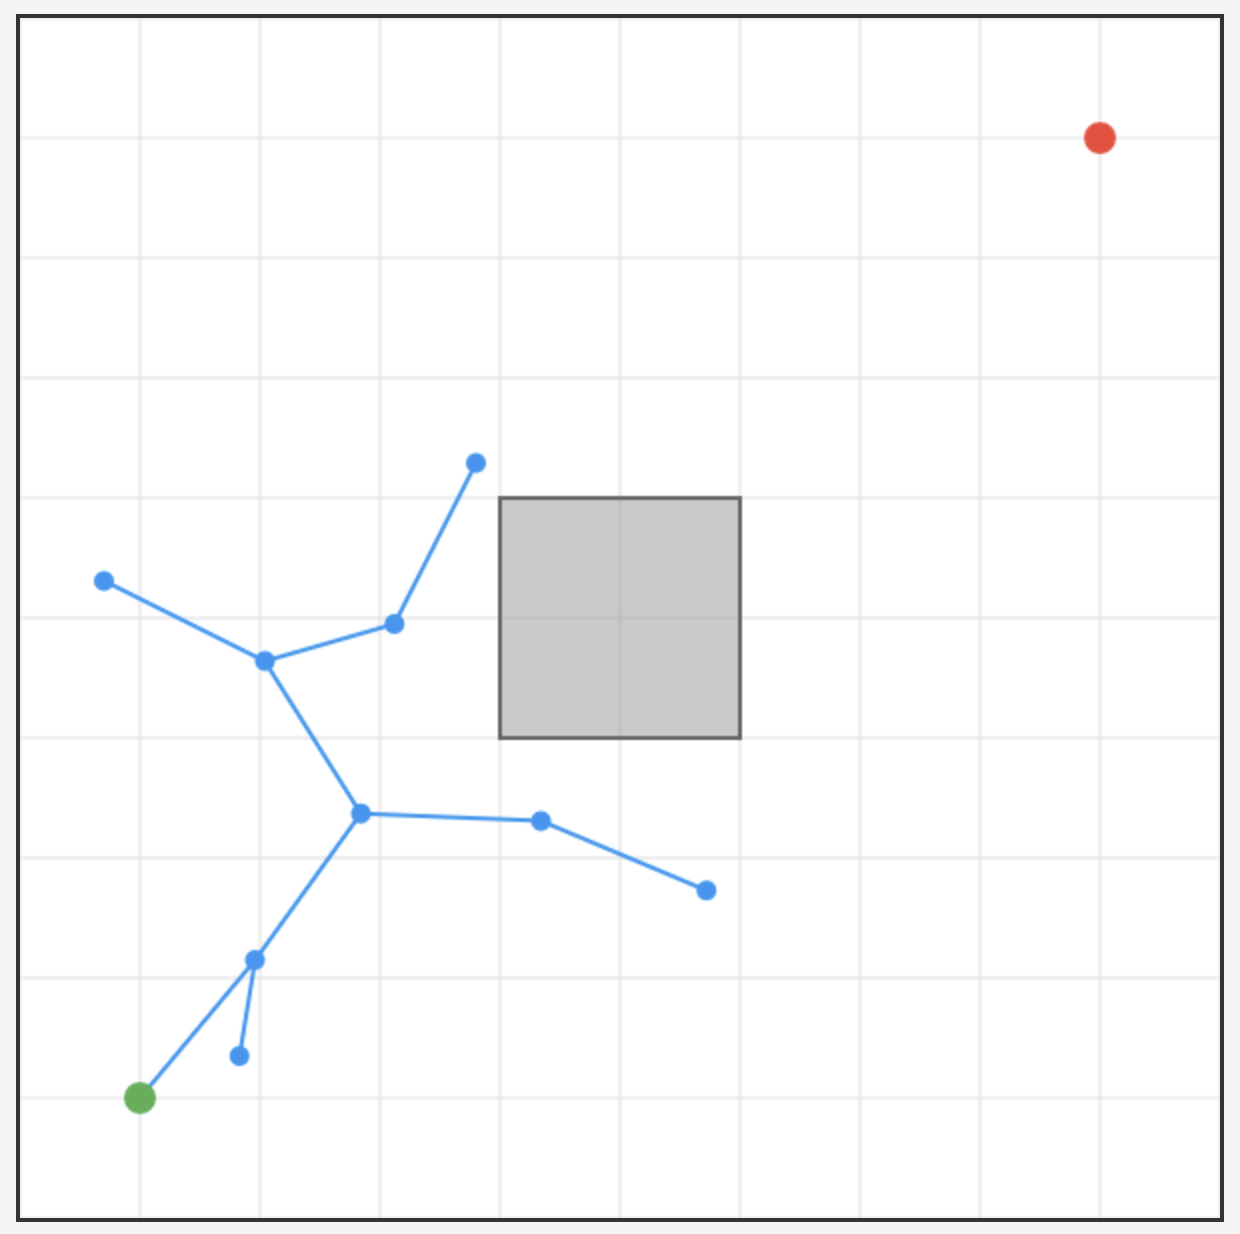
\includegraphics[width=0.7\textwidth]{rrt_growth.png}
    \caption{RRT after 10 iterations. Nodes are shown in blue, valid edges in black, the obstacle in gray, and start/goal in green/red.}
    \label{fig:rrt_growth}
\end{figure}

\textbf{Discussion.}
The tree expands systematically from the start toward unexplored regions of the workspace, demonstrating the RRT’s characteristic space-filling behavior.  
Only one attempted extension (Iteration 5) intersects the obstacle and is therefore rejected. After ten iterations, the tree contains nine valid edges and ten nodes, covering much of the lower-left to mid-right workspace.

The simulated results highlight how local collision constraints restrict branch expansion near the obstacle region and how random sampling ensures broad workspace coverage even with a small number of iterations.

% Problem 2(b): Goal bias and step size analysis

\subsection{Goal bias and step size analysis}

\subsubsection*{Question 1: Effect of increasing $p_{\text{goal}}$}

\textbf{(i) Speed of reaching the goal region:}

Increasing $p_{\text{goal}}$ \textbf{increases the speed} of reaching the goal. A higher goal bias means the algorithm samples the goal location more frequently, which directly pulls the tree toward the goal. This creates more edges pointing in the goal direction, accelerating convergence. In our simulation with $p_{\text{goal}} = 0.10$, no goal-biased samples occurred in 10 iterations. If we had set $p_{\text{goal}} = 0.50$, approximately 5 of the 10 samples would have been at the goal location $(9,9)$, creating direct paths toward the target.

\textbf{(ii) Diversity/coverage of explored space:}

Increasing $p_{\text{goal}}$ \textbf{decreases diversity and coverage} of the explored space. A higher goal bias creates a strong directional preference toward the goal, meaning the tree explores less of the overall workspace. The tree becomes more focused on reaching the goal and less exploratory of alternative regions. This reduces the coverage of the free space, which can be problematic if indirect paths are necessary.

\textbf{When can a large $p_{\text{goal}}$ hurt performance?}

A large goal bias can hurt performance in several scenarios:
\begin{itemize}
    \item \textbf{Narrow passages or complex obstacles:} When obstacles directly block the path between start and goal, an aggressive goal bias causes the tree to repeatedly attempt the same blocked direction, wasting samples without making progress toward finding alternative routes.
    
    \item \textbf{Exploration-dependent environments:} When the workspace requires exploring around obstacles before approaching the goal, a high $p_{\text{goal}}$ prevents the tree from discovering these necessary detours. In our example, if the obstacle were larger or positioned directly between start and goal, we would need to explore sideways or around before heading toward $(9,9)$.
    
    \item \textbf{Local minima:} The tree may get trapped in local configurations where all direct extensions toward the goal collide, and insufficient exploration prevents finding alternative paths.
\end{itemize}

The optimal $p_{\text{goal}}$ balances exploitation (moving toward the goal) with exploration (discovering diverse paths through the free space).

\subsubsection*{Question 2: Trade-offs in choosing $\eta$ (step size)}

The step size $\eta$ controls how far the tree extends toward each random sample. Choosing $\eta$ involves important trade-offs:

\textbf{If $\eta$ is much larger than typical obstacle feature sizes:}
\begin{itemize}
    \item \textbf{Problem:} Large steps may ``jump over'' narrow passages or small gaps in obstacles, causing the tree to miss valid paths that require precision navigation
    \item The tree cannot navigate through tight spaces because each extension is too coarse
    \item May fail to find feasible paths even when they exist
    \item \textbf{Example:} If $\eta = 5$ in our $10 \times 10$ workspace, a single step from $(1,1)$ could reach $(6,1)$, potentially jumping through the obstacle boundary without the collision checker detecting intermediate points properly
\end{itemize}

\textbf{If $\eta$ is much smaller than obstacle feature sizes:}
\begin{itemize}
    \item \textbf{Problem:} Very slow progress and inefficient exploration of the workspace
    \item Takes many iterations to make meaningful distance toward the goal
    \item Computational cost increases dramatically as more nodes are needed
    \item \textbf{Example:} If $\eta = 0.1$, traversing the diagonal distance from $(1,1)$ to $(9,9)$ (approximately 11.3 units) would require over 100 iterations just for the direct path, not accounting for obstacle avoidance
\end{itemize}

\textbf{Trade-off and rule of thumb:}

The optimal $\eta$ should be proportional to the smallest obstacle features or clearances that must be navigated:
\begin{itemize}
    \item \textbf{Rule of thumb:} Set $\eta \approx 0.5$ to $2$ times the minimum clearance or gap width
    \item Too large: miss narrow passages
    \item Too small: inefficient, slow convergence
    \item For our workspace with a $2 \times 2$ obstacle in a $10 \times 10$ space, $\eta = 1.5$ provides a reasonable balance between exploration efficiency and the ability to navigate around the obstacle
\end{itemize}

The step size should be large enough to make efficient progress but small enough to respect the geometric constraints of the environment.

\subsection{Collision Checking Resolution}

If the interpolation resolution $\delta$ is too coarse, the planner may miss collisions: two endpoints might be free while the segment between them crosses an obstacle. For example, an edge from $(3.5, 4.0)$ to $(6.5, 4.0)$ with $\delta = 2.0$ would only check the endpoints (both free), missing the collision in the middle where it passes through the obstacle.

If $\delta$ is too fine, computation becomes inefficient due to redundant checks. An edge of length 1.5 requires 6 checks with $\delta = 0.25$ but 150 checks with $\delta = 0.01$, providing minimal benefit.

A practical rule of thumb is to set $\delta$ between $\frac{1}{5}$ and $\frac{1}{2}$ of the minimum obstacle feature size. For our $2 \times 2$ obstacle, $\delta \approx 0.25$ is appropriate.

\subsection{Completeness and Planner Choice}

\textbf{(1)} Vanilla RRT is \textit{probabilistically complete}. If a collision-free path exists and the free space is connected, then as the number of samples $N \to \infty$, the probability that RRT finds a valid path approaches 1. Random sampling ensures that every region of free space will eventually be explored through the Voronoi bias property, which preferentially extends the tree toward unexplored regions.

\textbf{(2)} For a \textit{single-query} problem with tight time limits, RRT is preferred since it incrementally builds a tree from the start and can quickly reach the goal without precomputing a global roadmap. 

For a \textit{multi-query} setting where many start/goal pairs share the same workspace, PRM is preferred because its precomputed roadmap amortizes construction cost across many queries. After initial construction, each query only requires connecting the start/goal to the existing roadmap and running a graph search, which is much cheaper than rebuilding a tree from scratch for each query.

\subsection{RRT*}

RRT* is \textit{asymptotically optimal}, meaning that as the number of samples $N \to \infty$, the cost of the best path in the tree converges to the optimal path cost. 

It introduces a \textit{rewiring step}, in which nearby nodes within a shrinking radius are reconnected if the new connection through $q_{\text{new}}$ yields a lower cumulative cost. Additionally, when adding $q_{\text{new}}$, RRT* selects the best parent from nearby nodes rather than simply the nearest node. 

This local improvement process increases path quality at the expense of additional nearest-neighbor searches and collision checks per iteration, increasing computational cost compared to vanilla RRT. However, the resulting paths converge to optimality, whereas vanilla RRT paths can be arbitrarily suboptimal.

\section{Problem 3: Position Control and Impedance Control}
\subsection{PD Position Control}
\subsubsection*{Part 1: Closed-loop differential equation}

Given the PD controller:
\[
u = -K_p e - K_d \dot{x}
\]

Substituting into the dynamics $m\ddot{x} = u$:
\[
m\ddot{x} = -K_p e - K_d \dot{x}
\]

Since $e = x - x_d$ and $x_d$ is constant (desired position doesn't change), we have:
\begin{align*}
\dot{e} &= \dot{x} \\
\ddot{e} &= \ddot{x}
\end{align*}

Substituting $\ddot{x} = \ddot{e}$ and $\dot{x} = \dot{e}$ into the equation:
\[
m\ddot{e} = -K_p e - K_d \dot{e}
\]

Rearranging to standard form:
\[
\boxed{m\ddot{e} + K_d \dot{e} + K_p e = 0}
\]

This is the closed-loop differential equation in terms of error $e$.

\subsubsection*{Part 2: Characteristic equation and stability conditions}

To find the characteristic equation, we assume a solution of the form $e(t) = e^{\lambda t}$, where $\lambda$ is the characteristic root (eigenvalue).

Substituting into the differential equation:
\begin{align*}
m\lambda^2 e^{\lambda t} + K_d \lambda e^{\lambda t} + K_p e^{\lambda t} &= 0 \\
e^{\lambda t}(m\lambda^2 + K_d \lambda + K_p) &= 0
\end{align*}

Since $e^{\lambda t} \neq 0$, the characteristic equation is:
\[
\boxed{m\lambda^2 + K_d \lambda + K_p = 0}
\]

\textbf{Stability conditions:}

For the system to be asymptotically stable, both eigenvalues must have negative real parts. For a second-order polynomial $a\lambda^2 + b\lambda + c = 0$ to have roots with negative real parts, we require:
\begin{itemize}
\item All coefficients must be positive: $a > 0$, $b > 0$, $c > 0$
\end{itemize}

Applying this to our characteristic equation:
\begin{align*}
m &> 0 \quad \text{(always true, mass is positive)} \\
K_d &> 0 \\
K_p &> 0
\end{align*}

Therefore, the stability conditions are:
\[
\boxed{K_p > 0 \quad \text{and} \quad K_d > 0}
\]

\textbf{Why these conditions ensure stability:}

When both coefficients are positive, the characteristic polynomial satisfies the Routh-Hurwitz criterion for second-order systems. This guarantees that:
\begin{itemize}
\item If the roots are real, both are negative
\item If the roots are complex conjugates $\lambda = \alpha \pm j\omega$, then $\alpha < 0$ (negative real part)
\end{itemize}

In both cases, solutions decay exponentially: $e(t) \to 0$ as $t \to \infty$.

\subsubsection*{Part 3: Natural Frequency $\omega$ and Damping Ratio $\zeta$}
Given: $m = 2$ kg, $K_p = 10$, $K_d = 6$

The standard form of a second-order system is:
\[
\ddot{e} + 2\zeta\omega_n \dot{e} + \omega_n^2 e = 0
\]

Dividing our closed-loop equation by $m$:
\[
\ddot{e} + \frac{K_d}{m}\dot{e} + \frac{K_p}{m}e = 0
\]

Comparing coefficients:
\begin{align*}
\omega_n^2 &= \frac{K_p}{m} \\
2\zeta\omega_n &= \frac{K_d}{m}
\end{align*}

\textbf{Natural frequency:}
\[
\omega_n = \sqrt{\frac{K_p}{m}} = \sqrt{\frac{10}{2}} = \sqrt{5} \approx 2.236 \text{ rad/s}
\]

\textbf{Damping ratio:}

From $2\zeta\omega_n = \frac{K_d}{m}$:
\[
\zeta = \frac{K_d}{2m\omega_n} = \frac{K_d}{2\sqrt{mK_p}}
\]

Substituting values:
\[
\zeta = \frac{6}{2\sqrt{2 \cdot 10}} = \frac{6}{2\sqrt{20}} = \frac{6}{2 \cdot 2\sqrt{5}} = \frac{6}{4\sqrt{5}} = \frac{3}{2\sqrt{5}}
\]

Rationalizing the denominator:
\[
\zeta = \frac{3}{2\sqrt{5}} \cdot \frac{\sqrt{5}}{\sqrt{5}} = \frac{3\sqrt{5}}{10} \approx 0.671
\]

\textbf{Results:}
\[
\boxed{\omega_n = \sqrt{5} \approx 2.236 \text{ rad/s}, \quad \zeta = \frac{3\sqrt{5}}{10} \approx 0.671}
\]

\textbf{System classification:}

Since $0 < \zeta < 1$, the system is \textbf{underdamped}.

\subsection{Effect of Gravity and Feedforward Compensation}

\[
m\ddot{x} = u - mg,
\]
where $g = 9.81$ m/s$^2$.

\subsubsection*{Part 1: New closed-loop equation with gravity}

Using the same PD controller from part (a):
\[
u = -K_p e - K_d \dot{x}
\]

Substituting into the dynamics:
\[
m\ddot{x} = -K_p e - K_d \dot{x} - mg
\]

Since $e = x - x_d$ and $x_d$ is constant:
\begin{align*}
\dot{e} &= \dot{x} \\
\ddot{e} &= \ddot{x}
\end{align*}

Substituting:
\[
m\ddot{e} = -K_p e - K_d \dot{e} - mg
\]

Rearranging to standard form:
\[
\boxed{m\ddot{e} + K_d \dot{e} + K_p e = -mg}
\]

This is the new closed-loop equation with gravity. Note that the gravity term $-mg$ appears as a constant forcing term on the right-hand side.

\subsubsection*{Part 2: Steady-state error without gravity compensation}

At steady state, $\ddot{e} = 0$ and $\dot{e} = 0$. Substituting into the closed-loop equation:
\[
0 + 0 + K_p e_{ss} = -mg
\]

Solving for the steady-state error:
\[
\boxed{e_{ss} = -\frac{mg}{K_p}}
\]

This shows that the steady-state error is \textbf{nonzero} when there is no gravity compensation. The negative sign indicates that the actual position $x$ will be below the desired position $x_d$ by an amount $\frac{mg}{K_p}$, as the controller must maintain a constant error to balance the gravitational force.

\textbf{Physical interpretation:} The proportional term $-K_p e$ must generate a force equal to $mg$ to counteract gravity at steady state. This requires a nonzero position error.

\subsubsection*{Part 3: Gravity compensation eliminates steady-state error}

Add a gravity-compensating term to the control input:
\[
u = -K_p e - K_d \dot{x} + u_g
\]
where $u_g = mg$.

Substituting into the dynamics:
\[
m\ddot{x} = -K_p e - K_d \dot{x} + mg - mg = -K_p e - K_d \dot{x}
\]

The gravity terms cancel! Converting to error coordinates:
\[
m\ddot{e} = -K_p e - K_d \dot{e}
\]

Rearranging:
\[
\boxed{m\ddot{e} + K_d \dot{e} + K_p e = 0}
\]

This is identical to the gravity-free case from part (a). At steady state ($\ddot{e} = 0$, $\dot{e} = 0$):
\[
K_p e_{ss} = 0 \quad \Rightarrow \quad \boxed{e_{ss} = 0}
\]

\textbf{Conclusion:} The feedforward gravity compensation term $u_g = mg$ eliminates the steady-state error by directly counteracting the gravitational force, allowing the PD controller to regulate the position error to zero.

\subsection{Comparing Position and Impedance Control}
\subsubsection*{Part 1: Physical interpretation and comparison to position control}

\textbf{Physical interpretation of impedance control:}

Impedance control regulates the \textit{dynamic relationship} between position and force, rather than controlling position or force alone. It makes the robot behave like a mechanical system with specified mass, damping, and stiffness properties. The controller creates a virtual spring-damper-mass system that determines how the robot responds to external forces.

In impedance control, when an external force $F_{ext}$ is applied, the system responds according to:
\[
m\ddot{e} + K_d\dot{e} + Ke = F_{ext}
\]
where $K$ is the virtual stiffness, $K_d$ is the virtual damping, and $m$ is the virtual mass (which may differ from the actual physical mass).

\textbf{Key differences from pure position control:}

\begin{itemize}
    \item \textbf{Position control}: Rigidly drives the system to a desired position, treating deviations as errors to be eliminated. External forces are viewed as disturbances to be rejected. The system behaves like an infinitely stiff mechanism.
    
    \item \textbf{Impedance control}: Allows compliant interaction with the environment. The system can deviate from the desired position in response to external forces, with the amount of deviation determined by the virtual stiffness $K$. External forces cause controlled, predictable motion rather than being rejected.
    
    \item \textbf{Force response}: In position control, contact forces can become very large when interacting with rigid environments. In impedance control, the virtual stiffness limits contact forces and enables safe, stable interaction.
    
    \item \textbf{Control objective}: Position control aims to minimize position error regardless of forces. Impedance control aims to achieve a desired force-position relationship, trading position accuracy for force safety and interaction stability.
\end{itemize}

\subsubsection*{Part 2: Impact of K on System Behavior}

\textbf{If $K$ is very large (high stiffness):}

The system approaches \textbf{pure position control} behavior as the value of $K$ approaches $\infty$. 
The system becomes very rigid and resists external forces strongly, maintaining position despite disturbances. However, this can lead to large contact forces and potential instability or damage when interacting with stiff environments.
\newline
\textbf{If $K$ is very small (low stiffness, close to zero):}

The system exhibits \textbf{highly compliant behavior}. The system acts like a free mass with damping, easily displaced by external forces. Position tracking degrades significantly, but the robot can safely interact with its environment without generating large forces. The system behaves almost like it's ``floating'' with only damping providing resistance to motion.


\subsubsection*{Part 3: Application of different stiffness values}
There are varied use cases for the different stiffness parameter values that are chosen for the system. 
\textbf{High K values or stiff systems} are useful for tasks when a robot must perform high-accuracy operations like drilling circuit boards or milling metal parts. Other applications could potentially be Other examples include pick-and-place operations (accurate placement), inspection tasks (maintaining sensor position), and spot welding (precise electrode positioning). \textbf{Low K values or more compliant behavior} is better suited for 
a robot that works alongside humans (e.g., holding a workpiece while a human assembles components), as the low stiffness is more safe. If the human accidentally collides with the robot or needs to guide it manually it is more compliant to changing it's behavior and reduce chances of injury. 

\section{Problem 4: Camera Models and Callibration}

\subsection{Pinhole Camera Projection}

The pinhole camera model maps a 3D point $P = (X, Y, Z)^\top$ in the camera coordinate frame to homogeneous image coordinates via:
\[
\lambda \begin{bmatrix} u \\ v \\ 1 \end{bmatrix} = \begin{bmatrix} f_x & 0 & c_x \\ 0 & f_y & c_y \\ 0 & 0 & 1 \end{bmatrix} \begin{bmatrix} X \\ Y \\ Z \end{bmatrix} = K \begin{bmatrix} X \\ Y \\ Z \end{bmatrix},
\]
where $\lambda = Z$ in the pinhole model.

\subsubsection*{Part 1: Derive explicit formulas for $u$ and $v$}

Multiplying out the right-hand side:
\[
\lambda \begin{bmatrix} u \\ v \\ 1 \end{bmatrix} = \begin{bmatrix} f_x X + c_x Z \\ f_y Y + c_y Z \\ Z \end{bmatrix}
\]

This gives us three equations:
\begin{align}
\lambda u &= f_x X + c_x Z \label{eq:u_scaled} \\
\lambda v &= f_y Y + c_y Z \label{eq:v_scaled} \\
\lambda &= Z \label{eq:lambda}
\end{align}

From equation~\eqref{eq:lambda}, we know that $\lambda = Z$. Substituting into equation~\eqref{eq:u_scaled}:
\[
Z u = f_x X + c_x Z
\]

Dividing both sides by $Z$ (normalizing by $\lambda$):
\[
u = \frac{f_x X + c_x Z}{Z} = \frac{f_x X}{Z} + c_x
\]

Similarly, substituting $\lambda = Z$ into equation~\eqref{eq:v_scaled}:
\[
Z v = f_y Y + c_y Z
\]

Dividing both sides by $Z$:
\[
v = \frac{f_y Y + c_y Z}{Z} = \frac{f_y Y}{Z} + c_y
\]

\textbf{Final formulas:}
\[
\boxed{u = f_x \frac{X}{Z} + c_x}
\]
\[
\boxed{v = f_y \frac{Y}{Z} + c_y}
\]

These are the explicit projection formulas that map a 3D point $(X, Y, Z)$ to 2D pixel coordinates $(u, v)$ in the image plane.

\subsubsection*{Part 2: Compute $(u, v)$ in pixels}

Given:
\begin{itemize}
    \item $f_x = f_y = 800$ pixels
    \item $c_x = 320$ pixels
    \item $c_y = 240$ pixels
    \item $P = (0.1, 0.05, 1.0)$ meters = $(X, Y, Z) = (0.1, 0.05, 1.0)$
\end{itemize}

Using the formulas from Part 1:

\textbf{Computing $u$:}
\[
u = f_x \frac{X}{Z} + c_x = 800 \cdot \frac{0.1}{1.0} + 320 = 800 \cdot 0.1 + 320 = 80 + 320 = 400 \text{ pixels}
\]

\textbf{Computing $v$:}
\[
v = f_y \frac{Y}{Z} + c_y = 800 \cdot \frac{0.05}{1.0} + 240 = 800 \cdot 0.05 + 240 = 40 + 240 = 280 \text{ pixels}
\]

\textbf{Result:}
\[
\boxed{(u, v) = (400, 280) \text{ pixels}}
\]

This means the 3D point projects to pixel coordinates $(400, 280)$ in the image.

\subsubsection*{Part 3: Limiting behavior as $Z \to 0^+$ and $Z \to \infty$}

\textbf{Case 1: As $Z \to 0^+$ (point approaches camera center):}

As $Z \to 0^+$, the terms $\frac{X}{Z}$ and $\frac{Y}{Z}$ diverge to $\pm\infty$ (unless $X = Y = 0$):
\[
(u, v) \to (\pm\infty, \pm\infty)
\]

\textbf{Physical meaning:} Objects extremely close to the camera appear infinitely large due to extreme perspective. The projection becomes singular at $Z = 0$ (division by zero), where the point coincides with the pinhole itself. In practice, such points lie outside any real camera's field of view.

\textbf{Case 2: As $Z \to \infty$ (point moves far away):}

As $Z \to \infty$:
\[
u = f_x \frac{X}{Z} + c_x \to c_x, \quad v = f_y \frac{Y}{Z} + c_y \to c_y
\]

Therefore:
\[
\boxed{(u, v) \to (c_x, c_y) \text{ as } Z \to \infty}
\]

\textbf{Physical meaning:} Distant objects appear smaller and all points at infinity project to the principal point $(c_x, c_y)$, the vanishing point where the optical axis meets the image plane. This is why parallel lines (e.g., railroad tracks) appear to converge at the horizon.

\subsection{Extrinsic Parameters and Full Projection Matrix}

Suppose the camera frame is related to the world frame by a rotation $R \in SO(3)$ and translation $t \in \mathbb{R}^3$. In homogeneous coordinates:
\[
\begin{bmatrix} P_c \\ 1 \end{bmatrix} = \begin{bmatrix} R & t \\ 0 & 1 \end{bmatrix} \begin{bmatrix} P_w \\ 1 \end{bmatrix}
\]

\subsubsection*{Part 1: Derive the full projection equation}

Starting from part (a), we have the intrinsic projection:
\[
\lambda \begin{bmatrix} u \\ v \\ 1 \end{bmatrix} = K \begin{bmatrix} X_c \\ Y_c \\ Z_c \end{bmatrix}
\]
where $(X_c, Y_c, Z_c)$ are coordinates in the camera frame.

The extrinsic transformation relates world coordinates to camera coordinates:
\[
\begin{bmatrix} X_c \\ Y_c \\ Z_c \\ 1 \end{bmatrix} = \begin{bmatrix} R & t \\ 0 & 1 \end{bmatrix} \begin{bmatrix} X_w \\ Y_w \\ Z_w \\ 1 \end{bmatrix}
\]

This gives:
\[
\begin{bmatrix} X_c \\ Y_c \\ Z_c \end{bmatrix} = R \begin{bmatrix} X_w \\ Y_w \\ Z_w \end{bmatrix} + t
\]

Substituting into the intrinsic projection equation:
\[
\lambda \begin{bmatrix} u \\ v \\ 1 \end{bmatrix} = K \left( R \begin{bmatrix} X_w \\ Y_w \\ Z_w \end{bmatrix} + t \right)
\]

Expanding:
\[
\lambda \begin{bmatrix} u \\ v \\ 1 \end{bmatrix} = K R \begin{bmatrix} X_w \\ Y_w \\ Z_w \end{bmatrix} + K t
\]

To express this in homogeneous form, we can write:
\[
\lambda \begin{bmatrix} u \\ v \\ 1 \end{bmatrix} = K [R \mid t] \begin{bmatrix} X_w \\ Y_w \\ Z_w \\ 1 \end{bmatrix}
\]

where $[R \mid t]$ is the $3 \times 4$ matrix formed by concatenating $R$ (3×3) and $t$ (3×1).

\textbf{Full projection equation:}
\[
\boxed{\lambda \begin{bmatrix} u \\ v \\ 1 \end{bmatrix} = K [R \mid t] \begin{bmatrix} X_w \\ Y_w \\ Z_w \\ 1 \end{bmatrix}}
\]

The combined matrix $P = K [R \mid t]$ is a $3 \times 4$ projection matrix.

\textbf{Homogeneous normalization:}

After computing the matrix multiplication, we obtain:
\[
\lambda \begin{bmatrix} u \\ v \\ 1 \end{bmatrix} = \begin{bmatrix} p_1 \\ p_2 \\ p_3 \end{bmatrix}
\]

where $p_1, p_2, p_3$ are the three rows of the result. The homogeneous normalization divides by the third component:
\[
\lambda = p_3
\]

Therefore:
\[
u = \frac{p_1}{\lambda} = \frac{p_1}{p_3}, \quad v = \frac{p_2}{\lambda} = \frac{p_2}{p_3}
\]

This converts from homogeneous coordinates to pixel coordinates $(u, v)$.

\textbf{Alternative explicit form:}

Let $P_c = R P_w + t = (X_c, Y_c, Z_c)^\top$. Then from part (a):
\[
u = f_x \frac{X_c}{Z_c} + c_x, \quad v = f_y \frac{Y_c}{Z_c} + c_y
\]

where:
\[
\begin{bmatrix} X_c \\ Y_c \\ Z_c \end{bmatrix} = R \begin{bmatrix} X_w \\ Y_w \\ Z_w \end{bmatrix} + t
\]

\subsubsection*{Part 2: Geometric interpretation of $R$ and $t$}

\textbf{Rotation matrix $R$:}

$R \in SO(3)$ represents the \textit{orientation} of the camera frame relative to the world frame. Specifically, $R$ transforms vectors from world coordinates to camera coordinates by rotating them. The columns of $R$ are the world-frame representations of the camera's coordinate axes.

Alternatively, $R$ describes how the camera is rotated relative to the world. For example:
\begin{itemize}
    \item If $R = I$ (identity), the camera axes are aligned with the world axes
    \item $R$ captures effects like pan, tilt, and roll of the camera
\end{itemize}

\textbf{Translation vector $t$:}

$t \in \mathbb{R}^3$ represents the \textit{position} of the world origin as expressed in the camera coordinate frame. In other words, $t$ is the vector from the camera origin to the world origin, represented in camera coordinates.

\textbf{Note:} The camera center's position in world coordinates is $-R^\top t$ (since $R$ is orthogonal, $R^{-1} = R^\top$). This is because if we solve $0 = R P_w + t$ for $P_w$, we get $P_w = -R^{-1} t = -R^\top t$.

\textbf{Summary:}
\begin{itemize}
    \item $R$: Rotates world vectors into camera frame (camera orientation)
    \item $t$: Translates world origin to camera frame (position of world origin in camera coordinates)
    \item Together, $[R \mid t]$ forms the extrinsic parameters that relate world and camera frames
\end{itemize}

\subsection{Camera Callibration}
\subsubsection*{Part 1: 3D Stereo Reconstruction}
In stereo vision, depth $Z$ is recovered from disparity $d$ (the difference in pixel positions between left and right images) using:
\[
Z = \frac{f \cdot b}{d}
\]
where $f$ is the focal length and $b$ is the baseline (distance between cameras).

\textbf{Why calibration is critical:}

\begin{itemize}
    \item \textbf{Intrinsic parameters ($f_x, f_y, c_x, c_y$)}: Errors in focal length $f$ directly scale depth estimates. If the calibrated focal length is off by 5\%, depth estimates will be systematically wrong by 5\%. Incorrect principal points $(c_x, c_y)$ cause errors in computing disparity $d$, as the correspondence search assumes correct image centers.
    
    \item \textbf{Extrinsic parameters ($R, t$)}: The relative pose between left and right cameras must be known precisely. Even small rotation errors (e.g., 1° misalignment) cause incorrect rectification, leading to vertical disparities that violate the epipolar constraint and degrade matching accuracy. Translation errors directly affect the baseline $B$, causing proportional depth errors.
    
    \item \textbf{Mathematical impact}: If the true depth is $Z$ but we use incorrect focal length $\hat{f} = f + \Delta f$, the estimated depth becomes:
    \[
    \hat{Z} = \frac{\hat{f} \cdot b}{d} = \frac{(f + \Delta f) \cdot b}{d} = Z + \frac{\Delta f \cdot b}{d}
    \]
    The depth error grows linearly with $\Delta f$ and inversely with disparity $d$ (larger for distant objects).
\end{itemize}

\textbf{Consequences of poor calibration:} Inaccurate 3D point clouds lead to errors in obstacle detection, navigation, and manipulation. For instance, a robot might misjudge the distance to an object and collide with it or fail to grasp it.

\subsubsection*{Part 2: Visual servoing or eye-in-hand control}

Visual servoing controls robot motion by minimizing image-space errors $(\Delta u, \Delta v)$ between current and desired feature positions. The mapping from image error to Cartesian error $(\Delta X, \Delta Y, \Delta Z)$ requires the image Jacobian, which depends on camera parameters.

\textbf{Why calibration is critical:}

From the projection equations $u = f_x \frac{X}{Z} + c_x$ and $v = f_y \frac{Y}{Z} + c_y$, we can compute the image Jacobian relating Cartesian velocity to image velocity. Taking differentials:
\[
\Delta u \approx \frac{\partial u}{\partial X} \Delta X + \frac{\partial u}{\partial Y} \Delta Y + \frac{\partial u}{\partial Z} \Delta Z = \frac{f_x}{Z} \Delta X - \frac{f_x X}{Z^2} \Delta Z
\]
\[
\Delta v \approx \frac{\partial v}{\partial X} \Delta X + \frac{\partial v}{\partial Y} \Delta Y + \frac{\partial v}{\partial Z} \Delta Z = \frac{f_y}{Z} \Delta Y - \frac{f_y Y}{Z^2} \Delta Z
\]

The image Jacobian $J$ maps Cartesian motion to image motion:
\[
\begin{bmatrix} \Delta u \\ \Delta v \end{bmatrix} \approx J \begin{bmatrix} \Delta X \\ \Delta Y \\ \Delta Z \end{bmatrix}
\]

\textbf{Mathematical impact:}

\begin{itemize}
    \item \textbf{Intrinsic errors}: If $f_x$ or $f_y$ are incorrect, the Jacobian entries scale incorrectly, causing the robot to move too much or too little in response to image errors. For example, if the calibrated $\hat{f}_x = 1.1 f_x$ (10\% error), the robot will command 10\% smaller motions than needed, resulting in slow convergence or steady-state error.
    
    \item \textbf{Extrinsic errors}: The transformation $[R \mid t]$ relates camera frame motion to robot frame motion. If $R$ or $t$ are wrong, the computed Cartesian corrections $(\Delta X, \Delta Y, \Delta Z)$ will be in the wrong direction or magnitude, causing the robot to move incorrectly. For instance, a 5° rotation error could cause the robot to move perpendicular to the intended direction.
    
    \item \textbf{Depth dependence}: The Jacobian depends on depth $Z$. If depth is estimated incorrectly due to calibration errors, the commanded velocities will be wrong. Since terms like $\frac{f_x}{Z}$ appear, a 20\% error in $Z$ causes a 20\% error in the velocity gain.
\end{itemize}

\textbf{Consequences of poor calibration:} The robot may fail to align with the target, oscillate due to incorrect feedback gains, or become unstable. In precision tasks like assembly or surgical operations, even small calibration errors can cause task failure or damage.

\end{document}


